% Options for packages loaded elsewhere
\PassOptionsToPackage{unicode}{hyperref}
\PassOptionsToPackage{hyphens}{url}
%
\documentclass[
]{article}
\usepackage{amsmath,amssymb}
\usepackage{lmodern}
\usepackage{iftex}
\ifPDFTeX
  \usepackage[T1]{fontenc}
  \usepackage[utf8]{inputenc}
  \usepackage{textcomp} % provide euro and other symbols
\else % if luatex or xetex
  \usepackage{unicode-math}
  \defaultfontfeatures{Scale=MatchLowercase}
  \defaultfontfeatures[\rmfamily]{Ligatures=TeX,Scale=1}
\fi
% Use upquote if available, for straight quotes in verbatim environments
\IfFileExists{upquote.sty}{\usepackage{upquote}}{}
\IfFileExists{microtype.sty}{% use microtype if available
  \usepackage[]{microtype}
  \UseMicrotypeSet[protrusion]{basicmath} % disable protrusion for tt fonts
}{}
\makeatletter
\@ifundefined{KOMAClassName}{% if non-KOMA class
  \IfFileExists{parskip.sty}{%
    \usepackage{parskip}
  }{% else
    \setlength{\parindent}{0pt}
    \setlength{\parskip}{6pt plus 2pt minus 1pt}}
}{% if KOMA class
  \KOMAoptions{parskip=half}}
\makeatother
\usepackage{xcolor}
\usepackage[margin=1in]{geometry}
\usepackage{color}
\usepackage{fancyvrb}
\newcommand{\VerbBar}{|}
\newcommand{\VERB}{\Verb[commandchars=\\\{\}]}
\DefineVerbatimEnvironment{Highlighting}{Verbatim}{commandchars=\\\{\}}
% Add ',fontsize=\small' for more characters per line
\usepackage{framed}
\definecolor{shadecolor}{RGB}{248,248,248}
\newenvironment{Shaded}{\begin{snugshade}}{\end{snugshade}}
\newcommand{\AlertTok}[1]{\textcolor[rgb]{0.94,0.16,0.16}{#1}}
\newcommand{\AnnotationTok}[1]{\textcolor[rgb]{0.56,0.35,0.01}{\textbf{\textit{#1}}}}
\newcommand{\AttributeTok}[1]{\textcolor[rgb]{0.77,0.63,0.00}{#1}}
\newcommand{\BaseNTok}[1]{\textcolor[rgb]{0.00,0.00,0.81}{#1}}
\newcommand{\BuiltInTok}[1]{#1}
\newcommand{\CharTok}[1]{\textcolor[rgb]{0.31,0.60,0.02}{#1}}
\newcommand{\CommentTok}[1]{\textcolor[rgb]{0.56,0.35,0.01}{\textit{#1}}}
\newcommand{\CommentVarTok}[1]{\textcolor[rgb]{0.56,0.35,0.01}{\textbf{\textit{#1}}}}
\newcommand{\ConstantTok}[1]{\textcolor[rgb]{0.00,0.00,0.00}{#1}}
\newcommand{\ControlFlowTok}[1]{\textcolor[rgb]{0.13,0.29,0.53}{\textbf{#1}}}
\newcommand{\DataTypeTok}[1]{\textcolor[rgb]{0.13,0.29,0.53}{#1}}
\newcommand{\DecValTok}[1]{\textcolor[rgb]{0.00,0.00,0.81}{#1}}
\newcommand{\DocumentationTok}[1]{\textcolor[rgb]{0.56,0.35,0.01}{\textbf{\textit{#1}}}}
\newcommand{\ErrorTok}[1]{\textcolor[rgb]{0.64,0.00,0.00}{\textbf{#1}}}
\newcommand{\ExtensionTok}[1]{#1}
\newcommand{\FloatTok}[1]{\textcolor[rgb]{0.00,0.00,0.81}{#1}}
\newcommand{\FunctionTok}[1]{\textcolor[rgb]{0.00,0.00,0.00}{#1}}
\newcommand{\ImportTok}[1]{#1}
\newcommand{\InformationTok}[1]{\textcolor[rgb]{0.56,0.35,0.01}{\textbf{\textit{#1}}}}
\newcommand{\KeywordTok}[1]{\textcolor[rgb]{0.13,0.29,0.53}{\textbf{#1}}}
\newcommand{\NormalTok}[1]{#1}
\newcommand{\OperatorTok}[1]{\textcolor[rgb]{0.81,0.36,0.00}{\textbf{#1}}}
\newcommand{\OtherTok}[1]{\textcolor[rgb]{0.56,0.35,0.01}{#1}}
\newcommand{\PreprocessorTok}[1]{\textcolor[rgb]{0.56,0.35,0.01}{\textit{#1}}}
\newcommand{\RegionMarkerTok}[1]{#1}
\newcommand{\SpecialCharTok}[1]{\textcolor[rgb]{0.00,0.00,0.00}{#1}}
\newcommand{\SpecialStringTok}[1]{\textcolor[rgb]{0.31,0.60,0.02}{#1}}
\newcommand{\StringTok}[1]{\textcolor[rgb]{0.31,0.60,0.02}{#1}}
\newcommand{\VariableTok}[1]{\textcolor[rgb]{0.00,0.00,0.00}{#1}}
\newcommand{\VerbatimStringTok}[1]{\textcolor[rgb]{0.31,0.60,0.02}{#1}}
\newcommand{\WarningTok}[1]{\textcolor[rgb]{0.56,0.35,0.01}{\textbf{\textit{#1}}}}
\usepackage{longtable,booktabs,array}
\usepackage{calc} % for calculating minipage widths
% Correct order of tables after \paragraph or \subparagraph
\usepackage{etoolbox}
\makeatletter
\patchcmd\longtable{\par}{\if@noskipsec\mbox{}\fi\par}{}{}
\makeatother
% Allow footnotes in longtable head/foot
\IfFileExists{footnotehyper.sty}{\usepackage{footnotehyper}}{\usepackage{footnote}}
\makesavenoteenv{longtable}
\usepackage{graphicx}
\makeatletter
\def\maxwidth{\ifdim\Gin@nat@width>\linewidth\linewidth\else\Gin@nat@width\fi}
\def\maxheight{\ifdim\Gin@nat@height>\textheight\textheight\else\Gin@nat@height\fi}
\makeatother
% Scale images if necessary, so that they will not overflow the page
% margins by default, and it is still possible to overwrite the defaults
% using explicit options in \includegraphics[width, height, ...]{}
\setkeys{Gin}{width=\maxwidth,height=\maxheight,keepaspectratio}
% Set default figure placement to htbp
\makeatletter
\def\fps@figure{htbp}
\makeatother
\setlength{\emergencystretch}{3em} % prevent overfull lines
\providecommand{\tightlist}{%
  \setlength{\itemsep}{0pt}\setlength{\parskip}{0pt}}
\setcounter{secnumdepth}{-\maxdimen} % remove section numbering
\ifLuaTeX
  \usepackage{selnolig}  % disable illegal ligatures
\fi
\IfFileExists{bookmark.sty}{\usepackage{bookmark}}{\usepackage{hyperref}}
\IfFileExists{xurl.sty}{\usepackage{xurl}}{} % add URL line breaks if available
\urlstyle{same} % disable monospaced font for URLs
\hypersetup{
  pdftitle={PA1\_template.Rmd},
  pdfauthor={Chigo Chimoyo},
  hidelinks,
  pdfcreator={LaTeX via pandoc}}

\title{PA1\_template.Rmd}
\author{Chigo Chimoyo}
\date{2023-05-25}

\begin{document}
\maketitle

\hypertarget{loading-and-preprocessing-the-data}{%
\subsection{Loading and preprocessing the
data}\label{loading-and-preprocessing-the-data}}

The code below unzips the data file, loads it in R and thereafter
changes the class of the date column into a date class

\begin{Shaded}
\begin{Highlighting}[]
\FunctionTok{unzip}\NormalTok{(}\StringTok{"activity.zip"}\NormalTok{)}

\NormalTok{data }\OtherTok{\textless{}{-}} \FunctionTok{read.csv}\NormalTok{(}\StringTok{"activity.csv"}\NormalTok{)}

\NormalTok{data }\OtherTok{\textless{}{-}} \FunctionTok{transform}\NormalTok{(data, }\AttributeTok{date =} \FunctionTok{as.Date}\NormalTok{(data}\SpecialCharTok{$}\NormalTok{date))}
\end{Highlighting}
\end{Shaded}

\hypertarget{mean-and-total-number-of-steps-taken-per-day}{%
\subsection{Mean and Total number of steps taken per
day}\label{mean-and-total-number-of-steps-taken-per-day}}

The table below presents the total number of steps taken per each day
First 5 rows of the table

\begin{longtable}[]{@{}lr@{}}
\toprule()
date & steps \\
\midrule()
\endhead
2012-10-01 & 0 \\
2012-10-02 & 126 \\
2012-10-03 & 11352 \\
2012-10-04 & 12116 \\
2012-10-05 & 13294 \\
2012-10-06 & 15420 \\
\bottomrule()
\end{longtable}

The histogram below presents the total number of steps taken on each day

\begin{Shaded}
\begin{Highlighting}[]
  \FunctionTok{ggplot}\NormalTok{(step\_day, }\FunctionTok{aes}\NormalTok{(steps)) }\SpecialCharTok{+}
     \FunctionTok{geom\_histogram}\NormalTok{(}\AttributeTok{fill =} \StringTok{"darkred"}\NormalTok{)}\SpecialCharTok{+}
     \FunctionTok{labs}\NormalTok{(}\AttributeTok{title =} \StringTok{"Total number of steps per day"}\NormalTok{,}
              \AttributeTok{y =} \StringTok{"Count of steps"}\NormalTok{,}
              \AttributeTok{x =} \StringTok{"Steps"}\NormalTok{) }\SpecialCharTok{+}
     \FunctionTok{theme\_classic}\NormalTok{()}
\end{Highlighting}
\end{Shaded}

\begin{verbatim}
## `stat_bin()` using `bins = 30`. Pick better value with `binwidth`.
\end{verbatim}

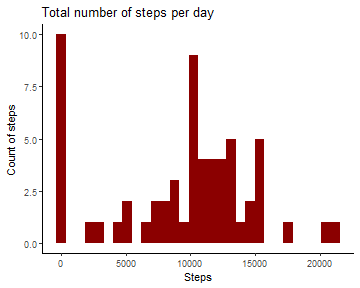
\includegraphics{PA1_template_files/figure-latex/histogram of steps per day-1.pdf}

The mean and median of the total number of steps taken per day

\begin{Shaded}
\begin{Highlighting}[]
\NormalTok{table }\OtherTok{\textless{}{-}} \FunctionTok{matrix}\NormalTok{(}\ConstantTok{NA}\NormalTok{, }\AttributeTok{ncol =} \DecValTok{2}\NormalTok{, }\AttributeTok{nrow =}  \DecValTok{2}\NormalTok{)}

\FunctionTok{colnames}\NormalTok{(table) }\OtherTok{\textless{}{-}} \FunctionTok{c}\NormalTok{(}\StringTok{"Computation"}\NormalTok{, }\StringTok{"Value"}\NormalTok{)}

\NormalTok{  table[}\DecValTok{1}\NormalTok{, ] }\OtherTok{\textless{}{-}} \FunctionTok{c}\NormalTok{(}\StringTok{"Mean"}\NormalTok{, }\FunctionTok{mean}\NormalTok{(step\_day}\SpecialCharTok{$}\NormalTok{steps, }\AttributeTok{na.rm =} \ConstantTok{TRUE}\NormalTok{))}
\NormalTok{  table[}\DecValTok{2}\NormalTok{, ] }\OtherTok{\textless{}{-}} \FunctionTok{c}\NormalTok{(}\StringTok{"Median"}\NormalTok{, }\FunctionTok{median}\NormalTok{(step\_day}\SpecialCharTok{$}\NormalTok{steps, }\AttributeTok{na.rm =} \ConstantTok{TRUE}\NormalTok{))}

\FunctionTok{kable}\NormalTok{(table, }\AttributeTok{format =} \StringTok{"simple"}\NormalTok{, }\AttributeTok{table.attr =} \StringTok{"style = \textquotesingle{}width:50\%;\textquotesingle{}"}\NormalTok{)}
\end{Highlighting}
\end{Shaded}

\begin{longtable}[]{@{}ll@{}}
\toprule()
Computation & Value \\
\midrule()
\endhead
Mean & 9354.22950819672 \\
Median & 10395 \\
\bottomrule()
\end{longtable}

\begin{Shaded}
\begin{Highlighting}[]
\NormalTok{ mean\_median }\OtherTok{\textless{}{-}}\NormalTok{  data }\SpecialCharTok{\%\textgreater{}\%} 
                      \FunctionTok{group\_by}\NormalTok{(date) }\SpecialCharTok{\%\textgreater{}\%} 
                      \FunctionTok{summarise}\NormalTok{( }\AttributeTok{mean =} \FunctionTok{mean}\NormalTok{(steps, }\AttributeTok{na.rm =} \ConstantTok{TRUE}\NormalTok{),}
                                   \AttributeTok{median =} \FunctionTok{median}\NormalTok{(steps, }\AttributeTok{na.rm =} \ConstantTok{TRUE}\NormalTok{))}

  \FunctionTok{kable}\NormalTok{(}\FunctionTok{head}\NormalTok{(mean\_median), }\AttributeTok{format =} \StringTok{"simple"}\NormalTok{)}
\end{Highlighting}
\end{Shaded}

\begin{longtable}[]{@{}lrr@{}}
\toprule()
date & mean & median \\
\midrule()
\endhead
2012-10-01 & NaN & NA \\
2012-10-02 & 0.43750 & 0 \\
2012-10-03 & 39.41667 & 0 \\
2012-10-04 & 42.06944 & 0 \\
2012-10-05 & 46.15972 & 0 \\
2012-10-06 & 53.54167 & 0 \\
\bottomrule()
\end{longtable}

\hypertarget{average-daily-activity-pattern}{%
\subsection{Average daily activity
pattern}\label{average-daily-activity-pattern}}

Time series plot of 5 minute intervals and average numbers of steps
taken, averaged across all days.

\begin{Shaded}
\begin{Highlighting}[]
\NormalTok{   temp }\OtherTok{\textless{}{-}} \FunctionTok{aggregate}\NormalTok{(data}\SpecialCharTok{$}\NormalTok{steps }\SpecialCharTok{\textasciitilde{}}\NormalTok{ data}\SpecialCharTok{$}\NormalTok{interval, }\AttributeTok{FUN =}\NormalTok{ mean)}
 
   \FunctionTok{colnames}\NormalTok{(temp) }\OtherTok{\textless{}{-}} \FunctionTok{c}\NormalTok{(}\StringTok{"interval"}\NormalTok{, }\StringTok{"avg\_steps"}\NormalTok{)}
  
\NormalTok{    y  }\OtherTok{\textless{}{-}}  \FunctionTok{max}\NormalTok{(temp}\SpecialCharTok{$}\NormalTok{avg\_steps)}
    
\NormalTok{    x }\OtherTok{\textless{}{-}}\NormalTok{ temp[temp}\SpecialCharTok{$}\NormalTok{avg\_steps }\SpecialCharTok{==} \FunctionTok{max}\NormalTok{(temp}\SpecialCharTok{$}\NormalTok{avg\_steps),}\DecValTok{1}\NormalTok{]}



\NormalTok{  data }\SpecialCharTok{\%\textgreater{}\%} 
      \FunctionTok{group\_by}\NormalTok{(interval) }\SpecialCharTok{\%\textgreater{}\%} 
      \FunctionTok{summarise}\NormalTok{(}\AttributeTok{average =} \FunctionTok{mean}\NormalTok{(steps, }\AttributeTok{na.rm =} \ConstantTok{TRUE}\NormalTok{)) }\SpecialCharTok{\%\textgreater{}\%} 
      \FunctionTok{ggplot}\NormalTok{(}\FunctionTok{aes}\NormalTok{(interval, average))}\SpecialCharTok{+}
          \FunctionTok{geom\_line}\NormalTok{()}\SpecialCharTok{+}
          \FunctionTok{labs}\NormalTok{( }\AttributeTok{title =}  \StringTok{"Average daily activity pattern"}\NormalTok{,}
                \AttributeTok{x =}  \StringTok{"5 min intervals"}\NormalTok{,}
                \AttributeTok{y =}  \StringTok{"Average steps daily"}\NormalTok{)}\SpecialCharTok{+}
          \FunctionTok{theme\_classic}\NormalTok{() }\SpecialCharTok{+}
          \FunctionTok{geom\_point}\NormalTok{(}\FunctionTok{aes}\NormalTok{(x,y), }\AttributeTok{cex =} \DecValTok{5}\NormalTok{, }\AttributeTok{color =} \StringTok{"darkred"}\NormalTok{)}
\end{Highlighting}
\end{Shaded}

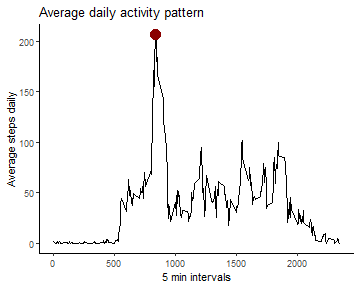
\includegraphics{PA1_template_files/figure-latex/Average daily activity patter-1.pdf}

The red point on the chart indicates the max average steps on 835 min
intervals

\hypertarget{imputing-missing-values}{%
\subsection{Imputing missing values}\label{imputing-missing-values}}

\begin{Shaded}
\begin{Highlighting}[]
\NormalTok{rows\_with\_NAs }\OtherTok{\textless{}{-}} \FunctionTok{sum}\NormalTok{(}\SpecialCharTok{!}\FunctionTok{complete.cases}\NormalTok{(data))}
\end{Highlighting}
\end{Shaded}

The data set has a total of 2304 missing variables.

These missing variables are replaced by the average number of steps
taken in time interval across all days using the code below.

A new dataset named data2 is created with all the missing values filled.

\begin{Shaded}
\begin{Highlighting}[]
\NormalTok{daily\_pattern }\OtherTok{\textless{}{-}}\NormalTok{ data }\SpecialCharTok{\%\textgreater{}\%} 
                    \FunctionTok{group\_by}\NormalTok{(interval) }\SpecialCharTok{\%\textgreater{}\%} 
                    \FunctionTok{summarise}\NormalTok{(}\AttributeTok{average =} \FunctionTok{mean}\NormalTok{(steps, }\AttributeTok{na.rm =} \ConstantTok{TRUE}\NormalTok{))}

\NormalTok{match }\OtherTok{\textless{}{-}}\NormalTok{ daily\_pattern}\SpecialCharTok{$}\NormalTok{average[}\FunctionTok{match}\NormalTok{(data}\SpecialCharTok{$}\NormalTok{interval, daily\_pattern}\SpecialCharTok{$}\NormalTok{interval)]}


\NormalTok{data2 }\OtherTok{\textless{}{-}} \FunctionTok{transform}\NormalTok{(data,}
                 \AttributeTok{steps =} \FunctionTok{ifelse}\NormalTok{(}\FunctionTok{is.na}\NormalTok{(data}\SpecialCharTok{$}\NormalTok{steps),}
                            \AttributeTok{yes =}\NormalTok{ match,}
                            \AttributeTok{no =}\NormalTok{ data}\SpecialCharTok{$}\NormalTok{steps))}
\end{Highlighting}
\end{Shaded}

Below is a histogram of the total number of steps taken each day.

\begin{Shaded}
\begin{Highlighting}[]
\NormalTok{data2 }\SpecialCharTok{\%\textgreater{}\%} 
  \FunctionTok{group\_by}\NormalTok{(date) }\SpecialCharTok{\%\textgreater{}\%} 
  \FunctionTok{summarize}\NormalTok{(}\AttributeTok{total\_steps =} \FunctionTok{sum}\NormalTok{(steps),}
            \AttributeTok{average\_steps =} \FunctionTok{mean}\NormalTok{(steps),}
            \AttributeTok{median\_steps =} \FunctionTok{median}\NormalTok{(steps)) }\SpecialCharTok{\%\textgreater{}\%} 
  \FunctionTok{ggplot}\NormalTok{(}\FunctionTok{aes}\NormalTok{(total\_steps))}\SpecialCharTok{+}
      \FunctionTok{geom\_histogram}\NormalTok{(}\AttributeTok{fill =} \StringTok{"darkred"}\NormalTok{)}\SpecialCharTok{+}
      \FunctionTok{labs}\NormalTok{( }\AttributeTok{title =}  \StringTok{"Plot 2; Total number of steps taken each day"}\NormalTok{,}
                \AttributeTok{x =}  \StringTok{"Steps freqency"}\NormalTok{,}
                \AttributeTok{y =}  \StringTok{"Steps count"}\NormalTok{)}\SpecialCharTok{+}
      \FunctionTok{theme\_classic}\NormalTok{()}
\end{Highlighting}
\end{Shaded}

\begin{verbatim}
## `stat_bin()` using `bins = 30`. Pick better value with `binwidth`.
\end{verbatim}

\begin{Shaded}
\begin{Highlighting}[]
\FunctionTok{ggplot}\NormalTok{(step\_day, }\FunctionTok{aes}\NormalTok{(steps)) }\SpecialCharTok{+}
   \FunctionTok{geom\_histogram}\NormalTok{(}\AttributeTok{fill =} \StringTok{"darkred"}\NormalTok{)}\SpecialCharTok{+}
   \FunctionTok{labs}\NormalTok{(}\AttributeTok{title =} \StringTok{"Plor 1; Total number of steps per day"}\NormalTok{,}
            \AttributeTok{y =} \StringTok{"Count of steps"}\NormalTok{,}
            \AttributeTok{x =} \StringTok{"Steps"}\NormalTok{) }\SpecialCharTok{+}
   \FunctionTok{theme\_classic}\NormalTok{()}
\end{Highlighting}
\end{Shaded}

\begin{verbatim}
## `stat_bin()` using `bins = 30`. Pick better value with `binwidth`.
\end{verbatim}

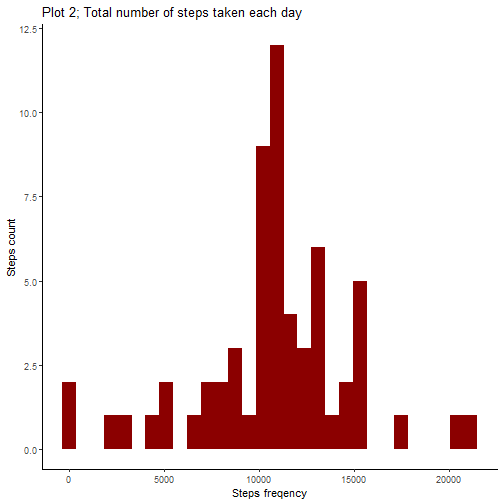
\includegraphics[width=0.48\linewidth]{PA1_template_files/figure-latex/histogram of steps taken eachday-1}
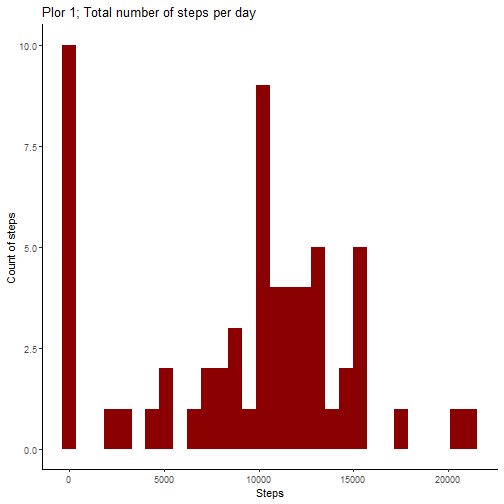
\includegraphics[width=0.48\linewidth]{PA1_template_files/figure-latex/histogram of steps taken eachday-2}

Plot 2, on the left side shows the total number of steps after inputting
the missing variables. whilst plot 1, on the right show the total number
of steps per day with the missing the variables.

As you may see, imputting the missing variables has changed the outlook
of the graph.

\hypertarget{difference-in-activity-pattern-between-weekday-and-weekends}{%
\subsection{Difference in activity pattern between weekday and
weekends}\label{difference-in-activity-pattern-between-weekday-and-weekends}}

Code below creates a new factor variable that indicates whether the day
is a weekday or a weekend.

\begin{Shaded}
\begin{Highlighting}[]
\NormalTok{days\_table }\OtherTok{\textless{}{-}} \FunctionTok{data.frame}\NormalTok{(}\AttributeTok{day =} \FunctionTok{c}\NormalTok{(}\StringTok{"Monday"}\NormalTok{, }\StringTok{"Tuesday"}\NormalTok{, }\StringTok{"Wednesday"}\NormalTok{, }
                                  \StringTok{"Thursday"}\NormalTok{, }\StringTok{"Friday"}\NormalTok{, }\StringTok{"Saturday"}\NormalTok{, }\StringTok{"Sunday"}\NormalTok{),}
                          \AttributeTok{mid\_end =} \FunctionTok{c}\NormalTok{(}\StringTok{"Weekday"}\NormalTok{,}\StringTok{"Weekday"}\NormalTok{,}\StringTok{"Weekday"}\NormalTok{,}\StringTok{"Weekday"}\NormalTok{,}\StringTok{"Weekday"}\NormalTok{, }
                                 \StringTok{"Weekend"}\NormalTok{, }\StringTok{"Weekend"}\NormalTok{))}

\NormalTok{data3 }\OtherTok{\textless{}{-}} \FunctionTok{transform}\NormalTok{(data2, }\AttributeTok{day =} \FunctionTok{weekdays}\NormalTok{(date))}

\NormalTok{day\_end }\OtherTok{\textless{}{-}} \FunctionTok{as.factor}\NormalTok{(days\_table}\SpecialCharTok{$}\NormalTok{mid\_end[(}\FunctionTok{match}\NormalTok{(data3}\SpecialCharTok{$}\NormalTok{day, days\_table}\SpecialCharTok{$}\NormalTok{day))])}

\NormalTok{data3 }\OtherTok{\textless{}{-}} \FunctionTok{cbind}\NormalTok{(data3, day\_end)}

\FunctionTok{kable}\NormalTok{(}\FunctionTok{head}\NormalTok{(data3), }\AttributeTok{format =} \StringTok{"simple"}\NormalTok{)}
\end{Highlighting}
\end{Shaded}

\begin{longtable}[]{@{}rlrll@{}}
\toprule()
steps & date & interval & day & day\_end \\
\midrule()
\endhead
1.7169811 & 2012-10-01 & 0 & Monday & Weekday \\
0.3396226 & 2012-10-01 & 5 & Monday & Weekday \\
0.1320755 & 2012-10-01 & 10 & Monday & Weekday \\
0.1509434 & 2012-10-01 & 15 & Monday & Weekday \\
0.0754717 & 2012-10-01 & 20 & Monday & Weekday \\
2.0943396 & 2012-10-01 & 25 & Monday & Weekday \\
\bottomrule()
\end{longtable}

Panel plot of a time series plot of the 5 minute interval and average
number of steps taken, averaged across all weekday days and weekend
days.

\begin{Shaded}
\begin{Highlighting}[]
\NormalTok{data3 }\SpecialCharTok{\%\textgreater{}\%} 
  \FunctionTok{group\_by}\NormalTok{(day\_end, interval) }\SpecialCharTok{\%\textgreater{}\%} 
  \FunctionTok{summarise}\NormalTok{(}\AttributeTok{avg =} \FunctionTok{mean}\NormalTok{(steps)) }\SpecialCharTok{\%\textgreater{}\%} 
  \FunctionTok{ggplot}\NormalTok{(}\FunctionTok{aes}\NormalTok{(interval, avg))}\SpecialCharTok{+}
      \FunctionTok{geom\_line}\NormalTok{()}\SpecialCharTok{+}
      \FunctionTok{labs}\NormalTok{( }\AttributeTok{title =}  \StringTok{"Time series plot"}\NormalTok{,}
                \AttributeTok{x =}  \StringTok{"5 minute interval"}\NormalTok{,}
                \AttributeTok{y =}  \StringTok{"Average number of steps"}\NormalTok{)}\SpecialCharTok{+}
      \FunctionTok{facet\_wrap}\NormalTok{(.}\SpecialCharTok{\textasciitilde{}}\NormalTok{ day\_end, }\AttributeTok{nrow =} \DecValTok{2}\NormalTok{) }\SpecialCharTok{+}
      \FunctionTok{theme}\NormalTok{(}\AttributeTok{panel.background =} \FunctionTok{element\_rect}\NormalTok{(}\AttributeTok{fill=}\StringTok{\textquotesingle{}transparent\textquotesingle{}}\NormalTok{))}
\end{Highlighting}
\end{Shaded}

\begin{verbatim}
## `summarise()` has grouped output by 'day_end'. You can override using the
## `.groups` argument.
\end{verbatim}

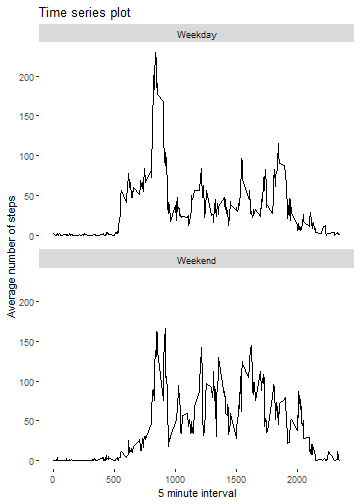
\includegraphics{PA1_template_files/figure-latex/time series plot-1.pdf}

\end{document}
